\section{Compiler generalities}\label{sec:aco:general}

    \subsection{Compiler}

        A compiler is a computer program that translates source code written in a high-level programming language into a target low-level programming language, allowing the computer to execute it. The target language can be assembly, object code, bytecode, or machine code.

        The compilation process involves several phases or passes that are implemented as modular components. These passes fall into three distinct classes: Front-end passes, Middle-end passes, and Back-end passes. The following sections will explore each category, providing detailed insights into their respective components, following the pipeline presented in~\Cref{fig:aco:general:compil}.

        \begin{figure}[hbt!]
                \begin{center}
                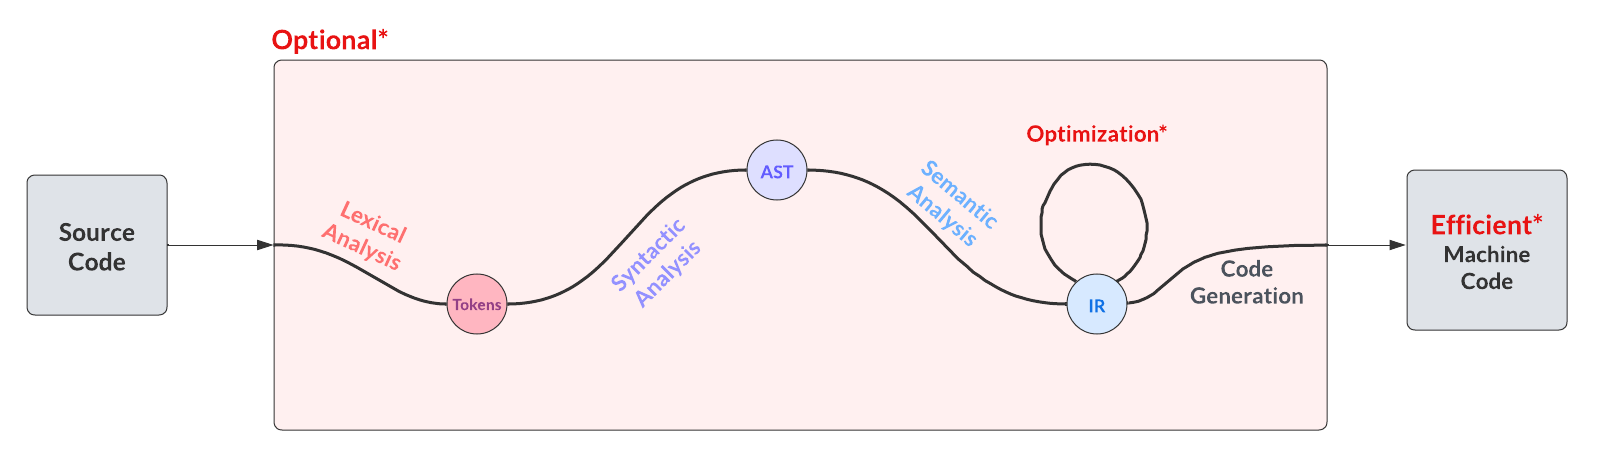
\includegraphics[width=.9\textwidth]{assets/images/compil.png}
                \end{center}
                \caption{Compilation Pipeline}%
                \label{fig:aco:general:compil}
            \end{figure}

    

    \subsection{Front-end Passes}
        Front-end compiler passes are designed for the specific source language of the program, involving essential analysis phases that every compiler must implement. These passes encompass lexical analysis, syntactic analysis, and semantic analysis. 

        \subsubsection{Lexical analysis}
            Lexical analysis, also known as lexing or scanning, involves taking the stream of characters that make up raw source code and breaking it down into tokens, as depicted in~\Cref{fig:aco:general:lexing}. These tokens can represent various elements, such as a character (e.g., ‘)’), a number (e.g., 123), a string (e.g., “hi”), an identifier (e.g., avg, min..), or a keyword (e.g., var).

            \begin{figure}[hbt!]
                \begin{center}
                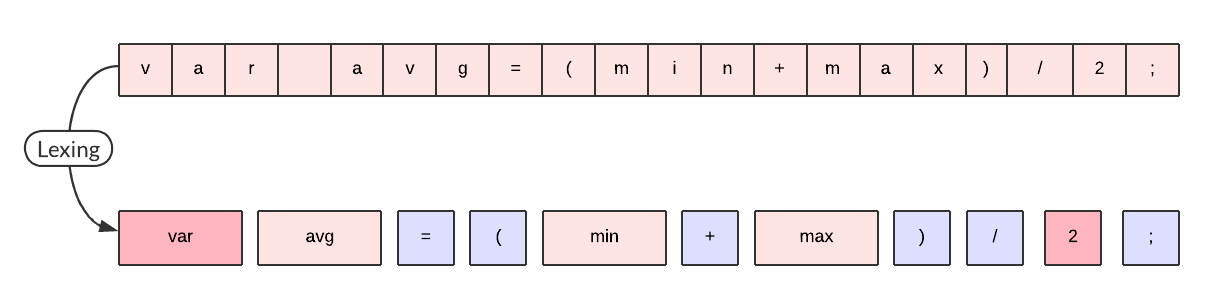
\includegraphics[width=.9\textwidth]{assets/images/lexing.png}
                \end{center}
                \caption{Lexical analysis}%
                \label{fig:aco:general:lexing}
            \end{figure}


        \subsubsection{Syntactic analysis}            
            Syntactic analysis, or parsing, is the stage where the sequence of tokens obtained from lexical analysis is processed. During this phase, the language's grammar is applied to the token sequence to construct a parse tree, commonly referred to as \gls{abb:ast}. This tree structure mirrors the nested structure of a program, as illustrated in~\Cref{fig:aco:general:ast}. The parser is responsible for detecting and reporting syntax errors.

            \begin{figure}[hbt!]
                \begin{center}
                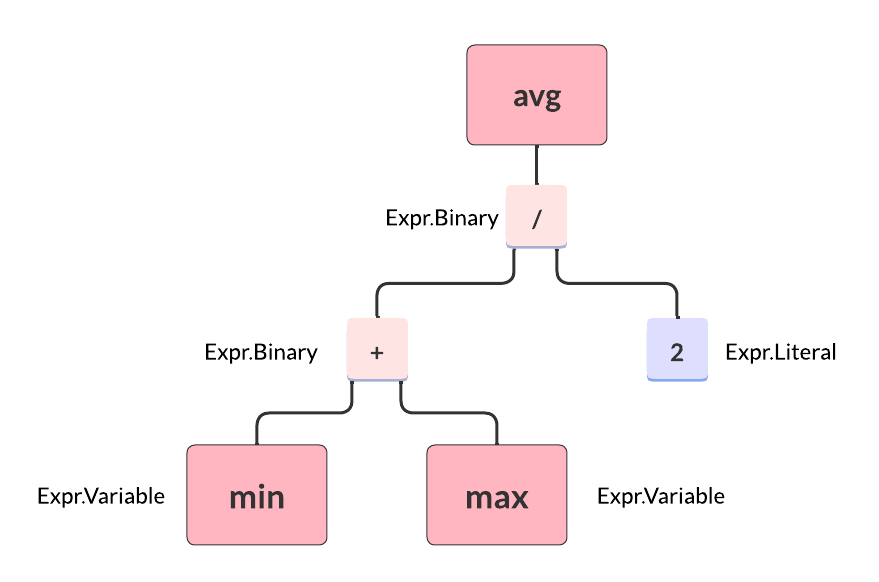
\includegraphics[width=.6\textwidth]{assets/images/ast.png}
                \end{center}
                \caption{Syntactic analysis}
                \label{fig:aco:general:ast}
            \end{figure}


        \subsubsection{Semantic analysis} 
            During this phase, semantic information is extracted from the generated \gls{abb:ast}. This involves capturing the scope of each identifier, and if the compiled language is statically typed, performing a type check. For dynamically typed languages, the type check is deferred until runtime.

            The gathered semantic insights can be stored as attributes within the \gls{abb:ast}. Another option is to use a symbol table, acting as a lookup table where identifiers serve as keys and their associated scopes as values. Alternatively, an optimal approach involves transforming the \gls{abb:ast} into a new data structure that inherently expresses the semantics of the code.

            

    \subsection{Middle-end Passes}
        Applying middle-end compiler passes is a phase that operates independently of both the source and target languages. In this phase, the source code undergoes a conversion into an intermediate representation, setting the stage for key optimization processes. 

        \subsubsection{Intermediate representation generation}

            In a compilation pipeline, each component serves the purpose of organizing the user's code in a way that makes the next component simpler to implement. In the pipeline's front-end, representations are specific to the source language, while in the back-end, they align with the hardware architecture on which the program will run. Serving as a bridge between the two, \gls{abb:ir} is an independent format that the compiler employs to encode both the syntactic and semantic information of the code. This not only facilitates the application of transformations and optimizations but also simplifies the process of generating executable code.

            \gls{abb:ir}'s independence from specific source languages and target platforms enables broad compiler support. For instance, GCC accommodates a diverse array of languages (such as C, C++, Objective C, Ada 95, Fortran 77, and Pascal) and architectures (including 64- and 32-bit ARM, 64- and 32-bit x86\_64 and x86, and 64-bit PowerPC and SPARC).

            Examples of mostly used \gls{abb:ir}s include control flow graphs, static single-assignment (SSA), and three-address code.

        \subsubsection{Code Optimization}

            Code optimization is the process of making a program more efficient by applying transformations to its code. This results in a modified code that maintains the same semantics as the original, but is implemented in a more efficient manner. While not obligatory,  code optimization is a beneficial step that leverages the hardware architecture to accelerate code execution and, in some cases, reduce energy and memory consumption. Examples of optimizations include constant folding, dead code elimination, and loop optimizations (which will be elaborated on in the next section).

    \subsection{Back-end Passes}
        This phase is all about generating code instructions that a computer can understand and execute on its hardware.

        \subsubsection{Code generation}
            Code generation is the process of converting \gls{abb:ir} into a form of code that is runnable by the machine, which is usually a set of assembly-like instructions. The generated instructions may take the form of \textbf{Machine Code}, which can be directly loaded by the Operating System onto the chip for execution. However, it's important to note that machine code generation is architecture-specific, making it a hustle to implement.

            Alternatively, the generated instructions can be in \textbf{bytecode}, which is produced for a hypothetical machine known as a \gls{abb:vm}. This \gls{abb:vm} acts as a program emulating an imaginary chip that supports our specified virtual architecture during runtime. For instance, if we implement our \gls{abb:vm} in C, it enables us to execute our language on any platform equipped with a C compiler.
